%\documentclass[journal,12pt,onecolumn]{IEEEtran}
\documentclass[journal,12pt,twocolumn]{IEEEtran}
%
\usepackage{setspace}
\usepackage{gensymb}
%\doublespacing
\singlespacing

%\usepackage{graphicx}
%\usepackage{amssymb}
%\usepackage{relsize}
\usepackage[cmex10]{amsmath}
%\usepackage{amsthm}
%\interdisplaylinepenalty=2500
%\savesymbol{iint}
%\usepackage{txfonts}
%\restoresymbol{TXF}{iint}
%\usepackage{wasysym}
\usepackage{amsthm}
\usepackage{mathrsfs}
\usepackage{txfonts}
\usepackage{stfloats}
\usepackage{cite}
\usepackage{cases}
\usepackage{subfig}
%\usepackage{xtab}
\usepackage{longtable}
\usepackage{multirow}
%\usepackage{algorithm}
%\usepackage{algpseudocode}
\usepackage{enumitem}
\usepackage{mathtools}
\usepackage{tikz}
\usepackage{circuitikz}
\usepackage{verbatim}
\usepackage{hyperref}
%\usepackage{stmaryrd}
\usepackage{tkz-euclide} % loads  TikZ and tkz-base
%\usetkzobj{all}
\usepackage{listings}
    \usepackage{color}                                            %%
    \usepackage{array}                                            %%
    \usepackage{longtable}                                        %%
    \usepackage{calc}                                             %%
    \usepackage{multirow}                                         %%
    \usepackage{hhline}                                           %%
    \usepackage{ifthen}                                           %%
  %optionally (for landscape tables embedded in another document): %%
    \usepackage{lscape}     
\usepackage{multicol}
\usepackage{chngcntr}
\usepackage{iftex}
%\usepackage[latin9]{inputenc}
\usepackage{geometry}
\usepackage{bm}
%\geometry{verbose,tmargin=2cm,bmargin=3cm,lmargin=1.8cm,rmargin=1.5cm,headheight=2cm,headsep=2cm,footskip=3cm}
\usepackage{array}
\newcolumntype{L}[1]{>{\raggedright\let\newline\\\arraybackslash\hspace{0pt}}m{#1}}
\newcolumntype{C}[1]{>{\centering\let\newline\\\arraybackslash\hspace{0pt}}m{#1}}
\newcolumntype{R}[1]{>{\raggedleft\let\newline\\\arraybackslash\hspace{0pt}}m{#1}}

%\usepackage{graphicx}
%\usepackage{setspace}
%\usepackage{parskip}

\def \hsp {\hspace{3mm}}

\makeatletter

\providecommand{\tabularnewline}{\\}



\makeatother
\ifxetex
\usepackage[T1]{fontenc}
\usepackage{fontspec}
%\setmainfont[ Path = fonts/]{Sanskrit_2003.ttf}
\newfontfamily\nakulafont[Script=Devanagari,AutoFakeBold=2,Path = fonts/]{Nakula}
%\newfontfamily\liberationfont{Liberation Sans Narrow}
%\newfontfamily\liberationsansfont{Liberation Sans}
\fi
\usepackage{tikz}
\usepackage{xcolor}
%\usepackage{enumerate}

%\usepackage{wasysym}
%\newcounter{MYtempeqncnt}
\DeclareMathOperator*{\Res}{Res}
%\renewcommand{\baselinestretch}{2}
\renewcommand\thesection{\arabic{section}}
\renewcommand\thesubsection{\thesection.\arabic{subsection}}
\renewcommand\thesubsubsection{\thesubsection.\arabic{subsubsection}}

\renewcommand\thesectiondis{\arabic{section}}
\renewcommand\thesubsectiondis{\thesectiondis.\arabic{subsection}}
\renewcommand\thesubsubsectiondis{\thesubsectiondis.\arabic{subsubsection}}

% correct bad hyphenation here
\hyphenation{op-tical net-works semi-conduc-tor}
\def\inputGnumericTable{}                                 %%

\lstset{
language=tex,
frame=single, 
breaklines=true
}

%\begin{document}
%


\newtheorem{theorem}{Theorem}[section]
\newtheorem{problem}{Problem}
\newtheorem{proposition}{Proposition}[section]
\newtheorem{lemma}{Lemma}[section]
\newtheorem{corollary}[theorem]{Corollary}
\newtheorem{example}{Example}[section]
\newtheorem{definition}[problem]{Definition}
%\newtheorem{thm}{Theorem}[section] 
%\newtheorem{defn}[thm]{Definition}
%\newtheorem{algorithm}{Algorithm}[section]
%\newtheorem{cor}{Corollary}
\newcommand{\BEQA}{\begin{eqnarray}}
\newcommand{\EEQA}{\end{eqnarray}}
\newcommand{\define}{\stackrel{\triangle}{=}}
\bibliographystyle{IEEEtran}
%\bibliographystyle{ieeetr}
\providecommand{\mbf}{\mathbf}
\providecommand{\pr}[1]{\ensuremath{\Pr\left(#1\right)}}
\providecommand{\qfunc}[1]{\ensuremath{Q\left(#1\right)}}
\providecommand{\sbrak}[1]{\ensuremath{{}\left[#1\right]}}
\providecommand{\lsbrak}[1]{\ensuremath{{}\left[#1\right.}}
\providecommand{\rsbrak}[1]{\ensuremath{{}\left.#1\right]}}
\providecommand{\brak}[1]{\ensuremath{\left(#1\right)}}
\providecommand{\lbrak}[1]{\ensuremath{\left(#1\right.}}
\providecommand{\rbrak}[1]{\ensuremath{\left.#1\right)}}
\providecommand{\cbrak}[1]{\ensuremath{\left\{#1\right\}}}
\providecommand{\lcbrak}[1]{\ensuremath{\left\{#1\right.}}
\providecommand{\rcbrak}[1]{\ensuremath{\left.#1\right\}}}
\theoremstyle{remark}
\newtheorem{rem}{Remark}
\newcommand{\sgn}{\mathop{\mathrm{sgn}}}
\providecommand{\abs}[1]{\left\vert#1\right\vert}
\providecommand{\res}[1]{\Res\displaylimits_{#1}} 
\providecommand{\norm}[1]{\left\lVert#1\right\rVert}
%\providecommand{\norm}[1]{\lVert#1\rVert}
\providecommand{\mtx}[1]{\mathbf{#1}}
\providecommand{\mean}[1]{E\left[ #1 \right]}
\providecommand{\fourier}{\overset{\mathcal{F}}{ \rightleftharpoons}}
%\providecommand{\hilbert}{\overset{\mathcal{H}}{ \rightleftharpoons}}
%\providecommand{\system}{\overset{\mathcal{H}}{ \longleftrightarrow}}
\providecommand{\system}[1]{\overset{\mathcal{#1}}{ \longleftrightarrow}}
\providecommand{\gauss}[2]{\mathcal{N}\ensuremath{\left(#1,#2\right)}}
%
	%\newcommand{\solution}[2]{\textbf{Solution:}{#1}}
\newcommand{\solution}{\noindent \textbf{Solution: }}
\newcommand{\cosec}{\,\text{cosec}\,}
\newcommand{\sinc}{\,\text{sinc}\,}
\newcommand{\rect}{\,\text{rect}\,}
\providecommand{\dec}[2]{\ensuremath{\overset{#1}{\underset{#2}{\gtrless}}}}
\newcommand{\myvec}[1]{\ensuremath{\begin{pmatrix}#1\end{pmatrix}}}
\newcommand{\mydet}[1]{\ensuremath{\begin{vmatrix}#1\end{vmatrix}}}
\newcommand*{\permcomb}[4][0mu]{{{}^{#3}\mkern#1#2_{#4}}}
\newcommand*{\perm}[1][-3mu]{\permcomb[#1]{P}}
\newcommand*{\comb}[1][-1mu]{\permcomb[#1]{C}}
%\numberwithin{equation}{section}
\numberwithin{equation}{section}
%\numberwithin{problem}{section}
%\numberwithin{definition}{section}
\makeatletter
\@addtoreset{figure}{problem}
\makeatother
\let\StandardTheFigure\thefigure
\let\vec\mathbf
%\renewcommand{\thefigure}{\theproblem.\arabic{figure}}
\renewcommand{\thefigure}{\theproblem}
%\setlist[enumerate,1]{before=\renewcommand\theequation{\theenumi.\arabic{equation}}
%\counterwithin{equation}{enumi}
%\renewcommand{\theequation}{\arabic{subsection}.\arabic{equation}}
\vspace{3cm}
%\usepackage{babel}
\begin{document}
\begin{tabular}{L{6cm} C{5cm} R{5cm} }
	\definecolor{circleorange}{rgb}{1,0.17,0.08}
\definecolor{darkorange}{rgb}{1,0.27,0.1}
\definecolor{orange2}{rgb}{1,0.5,0.15}
\definecolor{orange3}{rgb}{1,0.65,0.25}
\definecolor{yellow1}{rgb}{0.95,0.77,0.2}
%\begin{tikzpicture}[scale=0.2,every node/.style={transform shape}]
\begin{tikzpicture}[scale=0.1,every node/.style={transform shape}]
\draw [fill=circleorange,circleorange] (5,10) circle (1.15); 
\fill [darkorange] (5.06,8) -- (5.06,2) -- (7.3,1.2) -- (7.3,8.8) -- (5.06,8);
\fill [darkorange] (4.94,8) -- (4.94,2) -- (2.7,1.2) -- (2.7,8.8) -- (4.94,8);
\fill [orange2]    (7.4,8.4) -- (7.4,1.6) -- (8.2,1.2) -- (8.2,8.8) -- (7.4,8.4);
\fill [orange2]    (2.6,8.4) -- (2.6,1.6) -- (1.8,1.2) -- (1.8,8.8) -- (2.6,8.4);
\fill [orange3]    (8.3,8.4) -- (8.3,1.6) -- (9.0,1.2) -- (9.0,8.8) -- (8.3,8.4);
\fill [orange3]    (1.7,8.4) -- (1.7,1.6) -- (1.0,1.2) -- (1.0,8.8) -- (1.7,8.4);
\fill [yellow1]    (9.1,8.4) -- (9.1,1.6) -- (9.7,1.2) -- (9.7,8.8) -- (9.1,8.4);
\fill [yellow1]    (0.9,8.4) -- (0.9,1.6) -- (0.3,1.2) -- (0.3,8.8) -- (0.9,8.4);
\ifxetex
\node [scale=2.1] at (5,-0.1)  {   {\bf {\nakulafont  भारतीय प्रौद्योगिकी संस्थान हैदराबाद }} };
\node [scale=1.8] at (5,-1.2) {   {\bf { Indian Institute of Technology Hyderabad}} };
%\node [scale=1.8] at (5,-1.2) {   {\bf {\liberationsansfont Indian Institute of Technology Hyderabad}} };
\fi
\end{tikzpicture}
% \includegraphics[scale=0.05]{logo_iith} \newline
& Assignments 
	&
	AI1110
\end{tabular}
\vspace{-6mm}
\begin{center}
%\includegraphics[scale=0.95]{Yellow-Line}

\begin{tikzpicture}
\definecolor{yellow1}{rgb}{0.95,0.77,0.2}
\draw[line width=0.75mm, yellow1] (0,0) -- (\textwidth,0);
\end{tikzpicture}
\par\end{center}
\section{Uniform Random Numbers}
Let $U$ be a uniform random variable between 0 and 1.
\begin{enumerate}[label=\thesection.\arabic*
,ref=\thesection.\theenumi]
\item Generate $10^6$ samples of $U$ using a C program and save into a file called uni.dat .
\\
\solution Download the following files and execute the  C program.
\begin{lstlisting}
wget https://github.com/Ritvik-Sai-C/Random_numbers/blob/main/1.1/exrand.c
wget https://github.com/Ritvik-Sai-C/Random_numbers/blob/main/1.1/coeffs.h
\end{lstlisting}
Use the below command in the terminal to run the code
\begin{lstlisting}
gcc exrand.c -lm
./a.out
\end{lstlisting}
%
\item
Load the uni.dat file into python and plot the empirical CDF of $U$ using the samples in uni.dat. The CDF is defined as
\begin{align}
F_{U}(x) = \pr{U \le x}
\end{align}
\\
\solution 
The graph \ref{fig:uni_cdf} is obtained by running the below code
\begin{lstlisting}
https://github.com/Ritvik-Sai-C/Random_numbers/blob/main/1.2/uni_cdf.py
\end{lstlisting}
.\\
'\\
.\\
.\\
Run the following command in the terminal to run the code
\begin{lstlisting}
python3 uni_cdf.py
\end{lstlisting}
\begin{figure}[h]
\centering
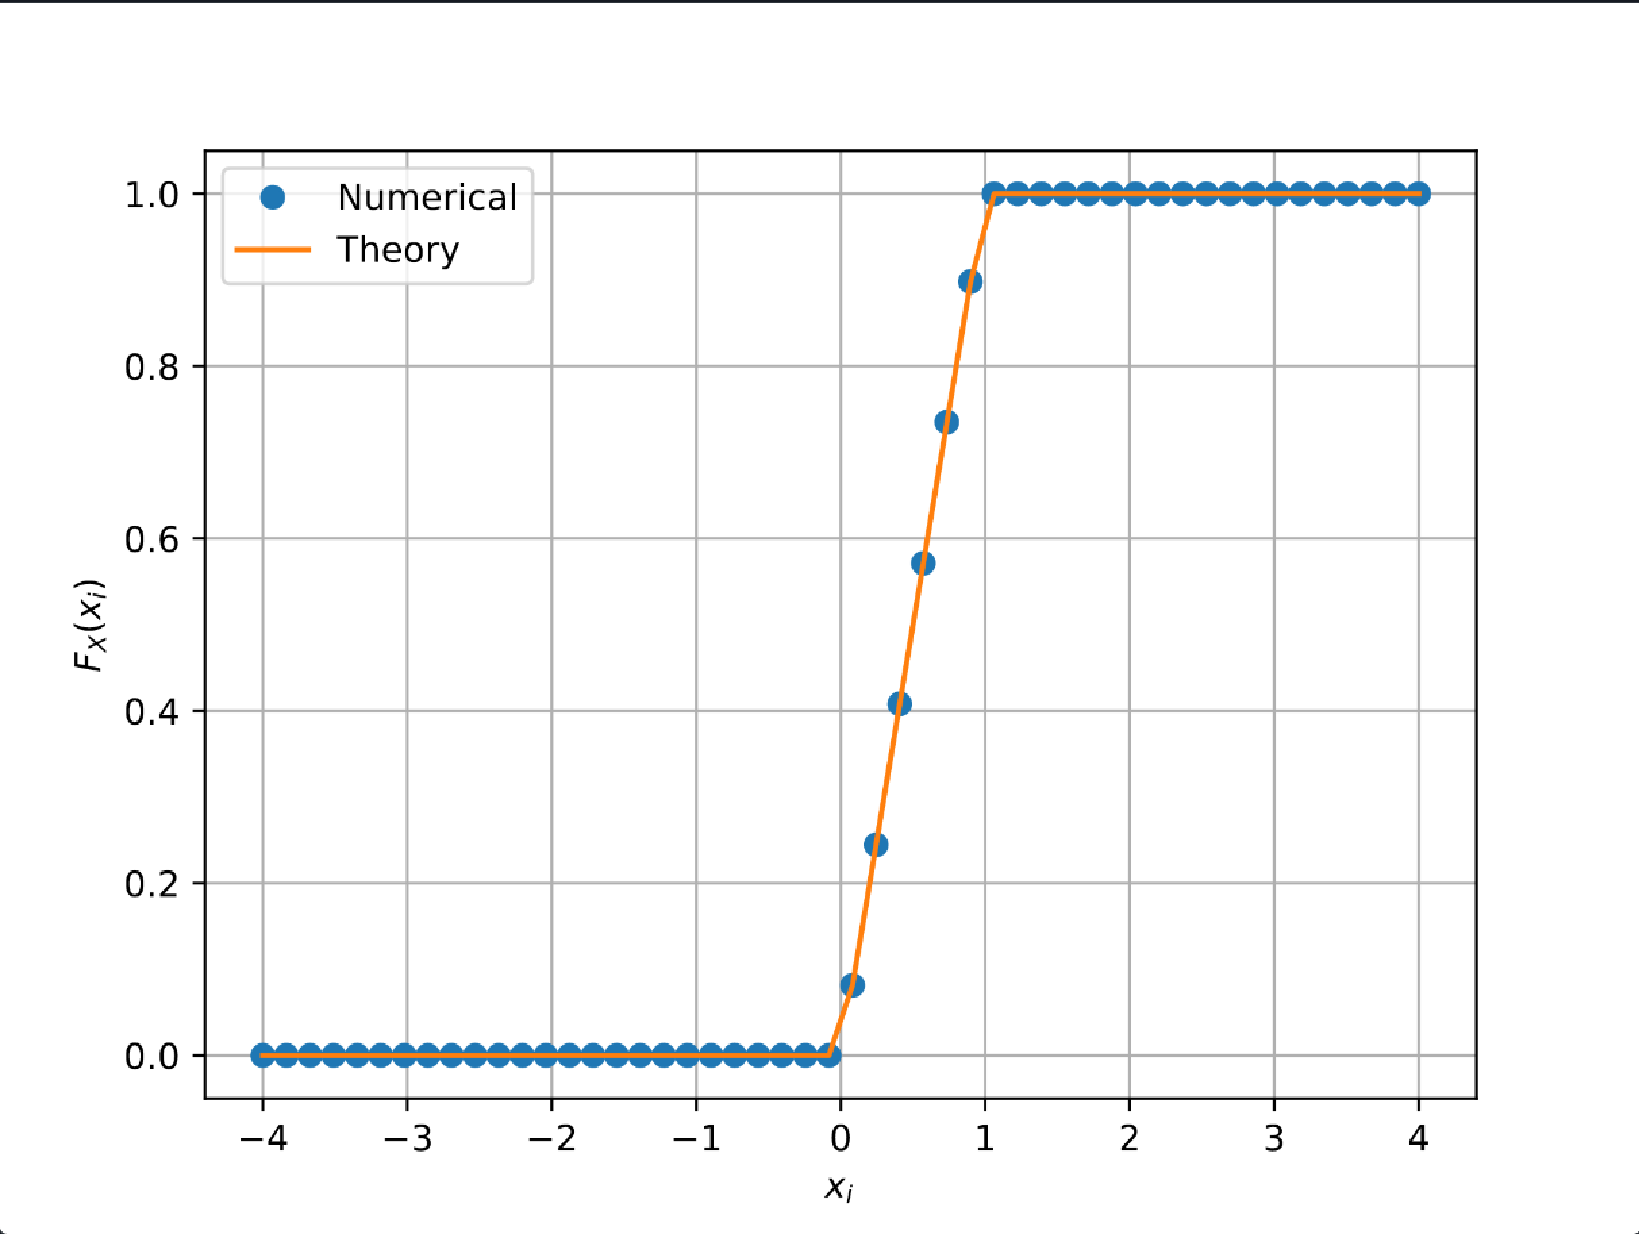
\includegraphics[width=\columnwidth]{./uni_cdf}
\caption{The CDF of $U$}
\label{fig:uni_cdf}
\end{figure}
%
\item
Find a  theoretical expression for $F_{U}(x)$.\
\solution
Since U is an uniform random variable distribution, $P_{U}(x_{i})=P_{U}(x_{j})=k$,$\forall i,j$\
	CDF of $P_{U}(x)$=$F_{U}(x)$\
	\begin{align}
	=\int P_{U}(x) dx\\
	=\int k dx\\
  \text{wkt} \int_{0}^{1} kdx=1\\
  \therefore k=1\\
  \therefore F_{U}(x)=x
	\end{align}	
\item
The mean of $U$ is defined as
%
\begin{equation}
E\sbrak{U} = \frac{1}{N}\sum_{i=1}^{N}U_i
\end{equation}
%
and its variance as
%
\begin{equation}
\text{var}\sbrak{U} = E\sbrak{U- E\sbrak{U}}^2 
\end{equation}
Write a C program to  find the mean and variance of $U$. \\
\solution
\begin{lstlisting}
wget https://github.com/Ritvik-Sai-C/Random_numbers/blob/main/1.4/mean_var.c
\end{lstlisting}
Use below command to run file,
\begin{lstlisting}
gcc mean_var.c -lm
./a.out
\end{lstlisting}
running the code gives us Mean =0.500137 , Variance =0.083251
\item Verify your result theoretically given that
\end{enumerate}
%
\begin{equation}
E\sbrak{U^k} = \int_{-\infty}^{\infty}x^kdF_{U}(x)
\end{equation}
\begin{align}
&dF_{U}(x)=dx\\
&\therefore E[U^k]=\int_{-\infty}^{\infty} x^k dx\\
&E[U]=\int_{0}^{1} x dx=\frac{1}{2}\\
&E[U^2]=\int_{0}^{1} x^2 dx=\frac{1}{3}\\
&\because P_{X}(x)=0 ,\forall x \in (1,\infty)\cap (-\infty,0)\\
&Var(X)=E[U^2]-(E[U])^2=\frac{1}{3}-\frac{1}{4}=\frac{1}{12}
\end{align}
\section{Central Limit Theorem}
%
\begin{enumerate}[label=\thesection.\arabic*
,ref=\thesection.\theenumi]
%
\item
Generate $10^6$ samples of the random variable
%
\begin{equation}
X = \sum_{i=1}^{12}U_i -6
\end{equation}
%
using a C program, where $U_i, i = 1,2,\dots, 12$ are  a set of independent uniform random variables between 0 and 1
and save in a file called gau.dat
\\
\solution
\begin{lstlisting}
wget https://github.com/Ritvik-Sai-C/Random_numbers/blob/main/1.1/exrand.c
wget https://github.com/Ritvik-Sai-C/Random_numbers/blob/main/1.1/coeffs.h
\end{lstlisting}
Running the above codes generates uni.dat and gau.dat file.
Use the command 
\begin{lstlisting}
gcc exrand.c -lm
.\a.out
\end{lstlisting}
%
\item
Load gau.dat in python and plot the empirical CDF of $X$ using the samples in gau.dat. What properties does a CDF have?
\\
\solution 
The CDF of $X$ is plotted in \ref{fig:gau_cdf},Properties of the CDF:
\begin{itemize}
\item $\Phi(x)=P(Z \leq x)= \frac{1}{\sqrt{2 \pi}} \int_{-\infty}^{x}\exp\left\{-\frac{u^2}{2}\right\} du$
\item $\lim \limits_{x\rightarrow \infty} \Phi(x)=1, \hspace{5pt} \lim \limits_{x\rightarrow -\infty} \Phi(x)=0$
\item  $\Phi(0)=\frac{1}{2}$
\item  $\Phi(-x)=1-\Phi(x)$
\end{itemize}
\begin{figure}[h]
\centering
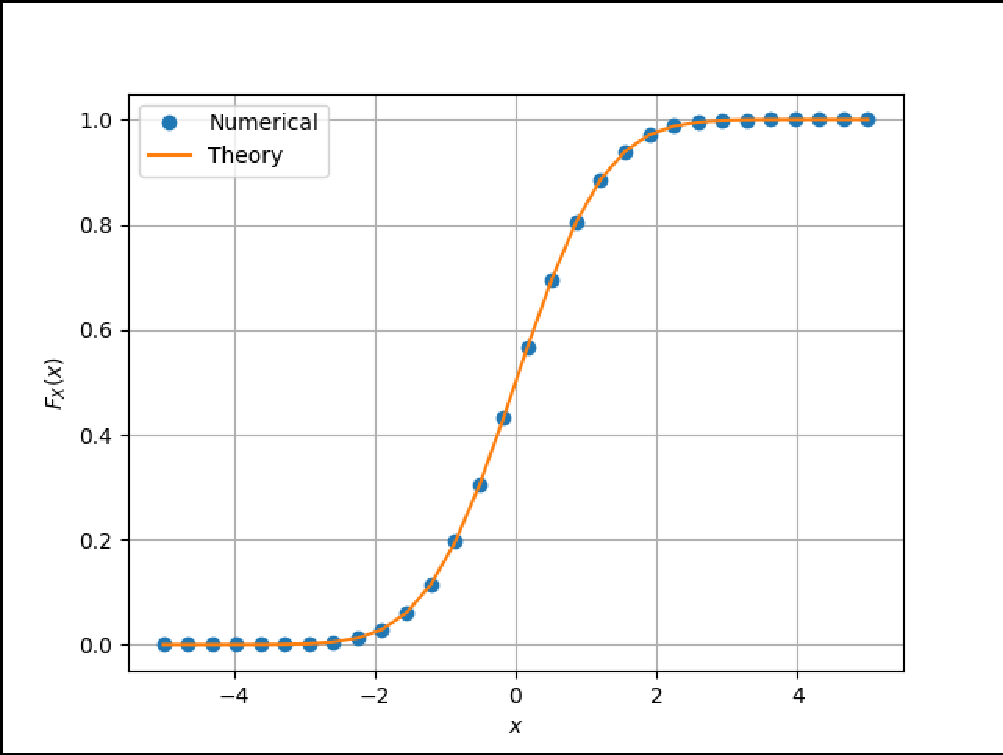
\includegraphics[width=\columnwidth]{./gau_cdf}
\caption{The CDF of $X$}
\label{fig:gau_cdf}
\end{figure}
\item
Load gau.dat in python and plot the empirical PDF of $X$ using the samples in gau.dat. The PDF of $X$ is defined as
\begin{align}
p_{X}(x) = \frac{d}{dx}F_{X}(x)
\end{align}
What properties does the PDF have?
\\
\begin{figure}[h]
\centering
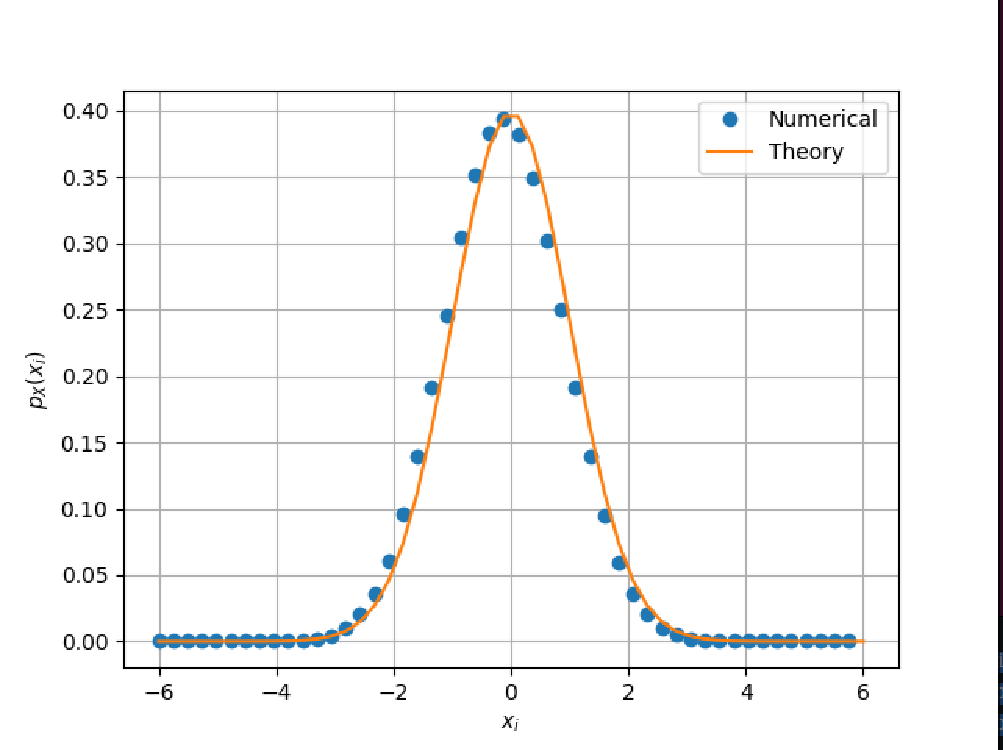
\includegraphics[width=\columnwidth]{./gauss_pdf}
\caption{The PDF of $X$}
\label{fig:gauss_pdf}
\end{figure}
\\
\solution The PDF of $X$ is plotted in \ref{fig:gauss_pdf} using the code below
\begin{lstlisting}
https://github.com/Ritvik-Sai-C/Random_numbers/blob/main/2.3/gauss_pdf.py
\end{lstlisting}
Use the below command to run the code:
\begin{lstlisting}
python3 pdf.py
\end{lstlisting}
Properties of PDF:
\begin{itemize}
\item PDF is symmetric about $x=0$\
\item graph is bell shaped\
\item mean of graph is situated at the apex point of the bell\
\end{itemize}
\item Find the mean and variance of $X$ by writing a C program.\\
\solution
Running the below code gives Mean = -0.000417 Variance= 0.999902
 \begin{lstlisting}
https://github.com/Ritvik-Sai-C/Random_numbers/blob/main/2.4/mean_var(gau).c
\end{lstlisting}
Command used:
\begin{lstlisting}
gcc mean_var(gau).c -lm
./a.out
\end{lstlisting}
\item Given that 
\begin{align}
p_{X}(x) = \frac{1}{\sqrt{2\pi}}\exp\brak{-\frac{x^2}{2}}, -\infty < x < \infty,
\end{align}
repeat the above exercise theoretically.
%
\end{enumerate}
Given ,$p_{X}(x)=\frac{1}{\sqrt{2\pi}} e^{\frac{-x^2}{2}}$\
\begin{align}
 &E[x]=\int_{-\infty}^{\infty} x p_{X}(x) dx\\
 &=\int_{-\infty}^{\infty} \frac{1}{\sqrt{2 \pi}} x e^{-\frac{-x^2}{2}}\\
  &\because x e^{-\frac{-x^2}{2}} \text{is a odd function},\\
  \nonumber
   &E[x]=0\\
 &E[x^2]=\int_{-\infty}^{\infty} x^2 p_{X}(x) dx\\
 &=\int_{-\infty}^{\infty} \frac{1}{\sqrt{2\pi}} x(xe^{-\frac{-x^2}{2}}) dx
\end{align}
  Using integration by parts:
  \begin{align}
   \label{eq:eq1}
 & =x\int xe^{-\frac{-x^2}{2}} dx-\int\frac{d(x)}{dx} \int xe^{-\frac{-x^2}{2}}dx\\
 &I=\int x e^{-\frac{-x^2}{2}}\\
 &\text{Let} \frac{x^2}{2}=t \\
 &\implies x dx=dt\\
 &\implies =\int e^{-t} dt=-e^{-t} +c\\
 \label{eq:eq2}
 &\therefore \int x e^{-\frac{-x^2}{2}}=-e^{-\frac{-x^2}{2}} +c
 \end{align}
 Using \eqref{eq:eq2} in \eqref{eq:eq1}\
 \begin{align}
&= -x e^{-\frac{-x^2}{2}}+\int e^{-\frac{-x^2}{2}} dx\\
&\text{Also} ,\int_{-\infty}^{\infty} e^{-\frac{-x^2}{2}} dx=\sqrt{2 \pi} \\
&\therefore \text{substituting limits we get}, E[x^2]=1\\
 &Var(X)=E[x^2]-(E[x])^2=1-0
 \end{align}
\section{From Uniform to Other}
\begin{enumerate}[label=\thesection.\arabic*
,ref=\thesection.\theenumi]
%
\item
Generate samples of 
%
\begin{equation}
V = -2\ln\brak{1-U}
\end{equation}
%
and plot its CDF.\\ 
 \begin{figure}[h]
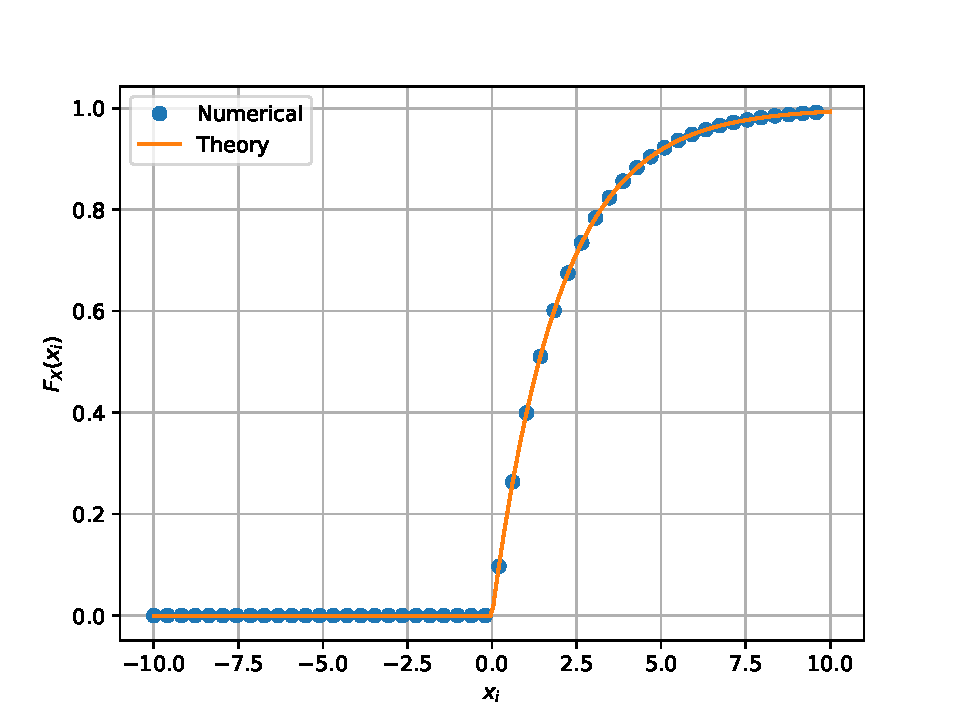
\includegraphics[width=0.5\textwidth]{V_cdf.pdf}
\caption{CDF for (3)}
\label{fig:V}
\end{figure}
\\ 
\solution
Running the below code generates samples of V from file uni.dat(U).
\begin{lstlisting}
https://github.com/Ritvik-Sai-C/Random_numbers/blob/main/3.1/V.py
\end{lstlisting}
Use the below command in the terminal to run the code:
\begin{lstlisting}
python3 V.py
\end{lstlisting}
 
Now these samples are used to plot \eqref{fig:V} by running the below code,
\begin{lstlisting}
https://github.com/Ritvik-Sai-C/Random_numbers/blob/main/3.1/V_cdf.py
\end{lstlisting}
Use the below command to run the code:
\begin{lstlisting}
python3 V_cdf.py
\end{lstlisting}
\item Find a theoretical expression for $F_V(x)$.
\begin{align}
 &F_{V}(x)=P(V \leq x)\\
 &=P(-2 ln(1-U) \leq x)\\
 &=P(1-e^{\frac{-x}{2}} \geq U)\\
 &P(U<x)=\int_{0}^{x} dx=x\\
 &\therefore P(1-e^{\frac{-x}{2}} \geq U)=1-e^{\frac{-x}{2}}, \forall x\geq 0 \\ 
 \nonumber
 \end{align}
%
%\item
%Generate the Rayleigh distribution from Uniform. Verify your result through graphical plots.
\end{enumerate}
\section{Triangular Distribution}
\begin{enumerate}[label=\thesection.\arabic*
,ref=\thesection.\theenumi]
%
\item Generate 
	\begin{align}
		T = U_1+U_2
	\end{align}
\solution 
Run the below code to generate T.dat
\begin{lstlisting}
https://github.com/Ritvik-Sai-C/Random_numbers/blob/main/4.1/T_gen_dat.c
\end{lstlisting}
Run the command below in the terminal 
\begin{lstlisting}
gcc T_gen_dat.c -lm
./a.out
\end{lstlisting}
\item Find the CDF of $T$.
\begin{align}
F_{T}(t)=P(T<t)
\\=P(U_1 +U_2 <t)
\end{align}
we know that $0\leq U_1 \leq 1$ and $0\leq U_2 \leq 1$\\
$\therefore 0\leq U_1 + U_2 \leq 2$, so\\
 $\forall t>2, P(U_1 +U_2 <t)=1$\\
 $\forall t<0, P(U_1 +U_2 <t)=0$\\
   for $0\leq t \leq 2$ let us split it into 2 cases, for $0 \leq t\leq 1$ and $1 <t \leq2$\\
    \begin{figure}[h]
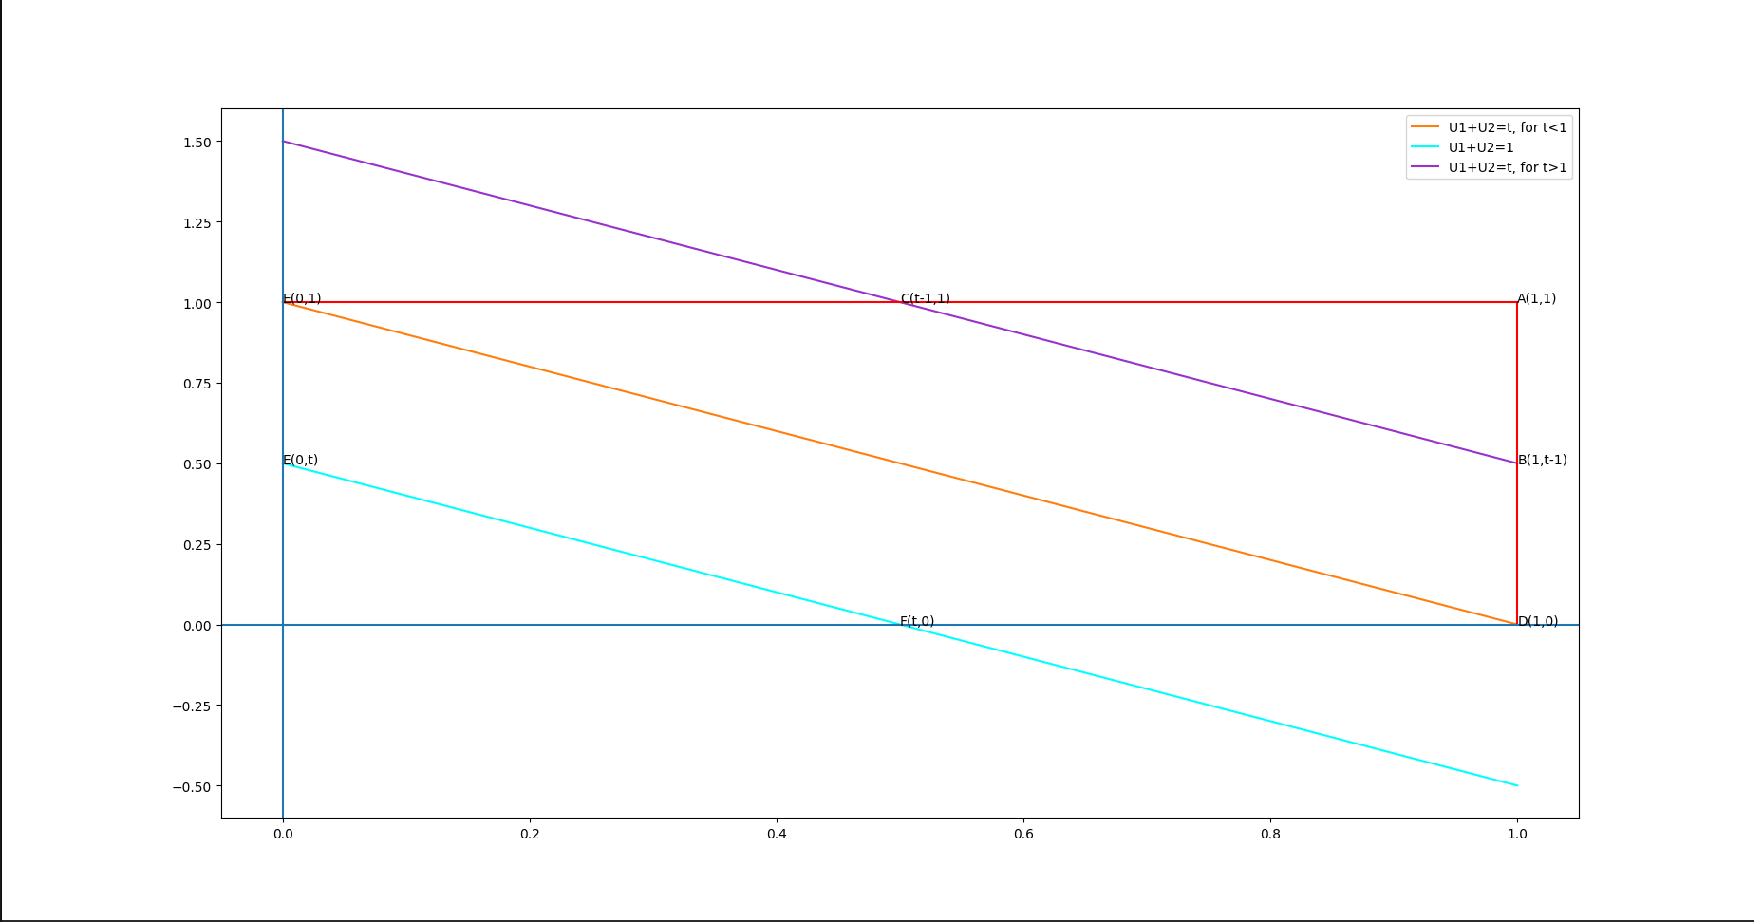
\includegraphics[width=0.5\textwidth]{T_plot}
\caption{Plot}
\label{fig:T_plot}
\end{figure}
\\
The above figure is produced by the following code
\begin{lstlisting}
https://github.com/Ritvik-Sai-C/Random_numbers/blob/main/4.2/T_plot.py
\end{lstlisting}
Run the following command in the terminal to run the code
\begin{lstlisting}
python3 T_plot.py
\end{lstlisting}
From Fig \eqref{fig:T_plot}
\begin{align}
&P(U_1+U_2<t, 0\leq t \leq 1)=\frac{ \Delta(EOF)}{\Delta(AEOD)}\\
&=\frac{t^2}{2}\\
&P(U_1+U_2<t, 1\leq t \leq 2)=\frac{\Delta(ABC)}{\Delta(AEOD)}\\
&=1-\frac{(2-t)^{2}}{2}\\
&\therefore F_{T}(t)=P(U_1 +U_2<t)=
\begin{cases}
0 & t<0\\
\frac{t^2}{2} & 0\leq t \leq 1\\
1-\frac{(2-t)^{2}}{2} & 1< t \leq 2\\
1 & t>2
\end{cases}
\end{align}
\item Find the PDF of $T$.\\
\solution 
\begin{align}
P_{T}(t)=\frac{d(F_{T}(t))}{dt}\\
\therefore P_{T}(t)=
\begin{cases}
0 & t<0\\
t & 0\leq t \leq 1\\
2-t  & 0< t \leq 2\\
0 & t>2 
\end{cases}    
\end{align}
\item Find the theoretical expressions for the PDF and CDF of $T$.
\\
\solution
\begin{align}
P_{T}(t)=
\begin{cases}
0 & t<0\\
t & 0\leq t \leq 1\\
2-t  & 0< t \leq 2\\
0 & t>2 
\end{cases} 
\\   
F_{T}(t)=
\begin{cases}
0 & t<0\\
\frac{t^2}{2} & 0\leq t \leq 1\\
1-\frac{(2-t)^{2}}{2} & 1< t \leq 2\\
1 & t>2
\end{cases}
\end{align}
\item Verify your results through a plot. 
\\
\solution 
 \begin{figure}[h]
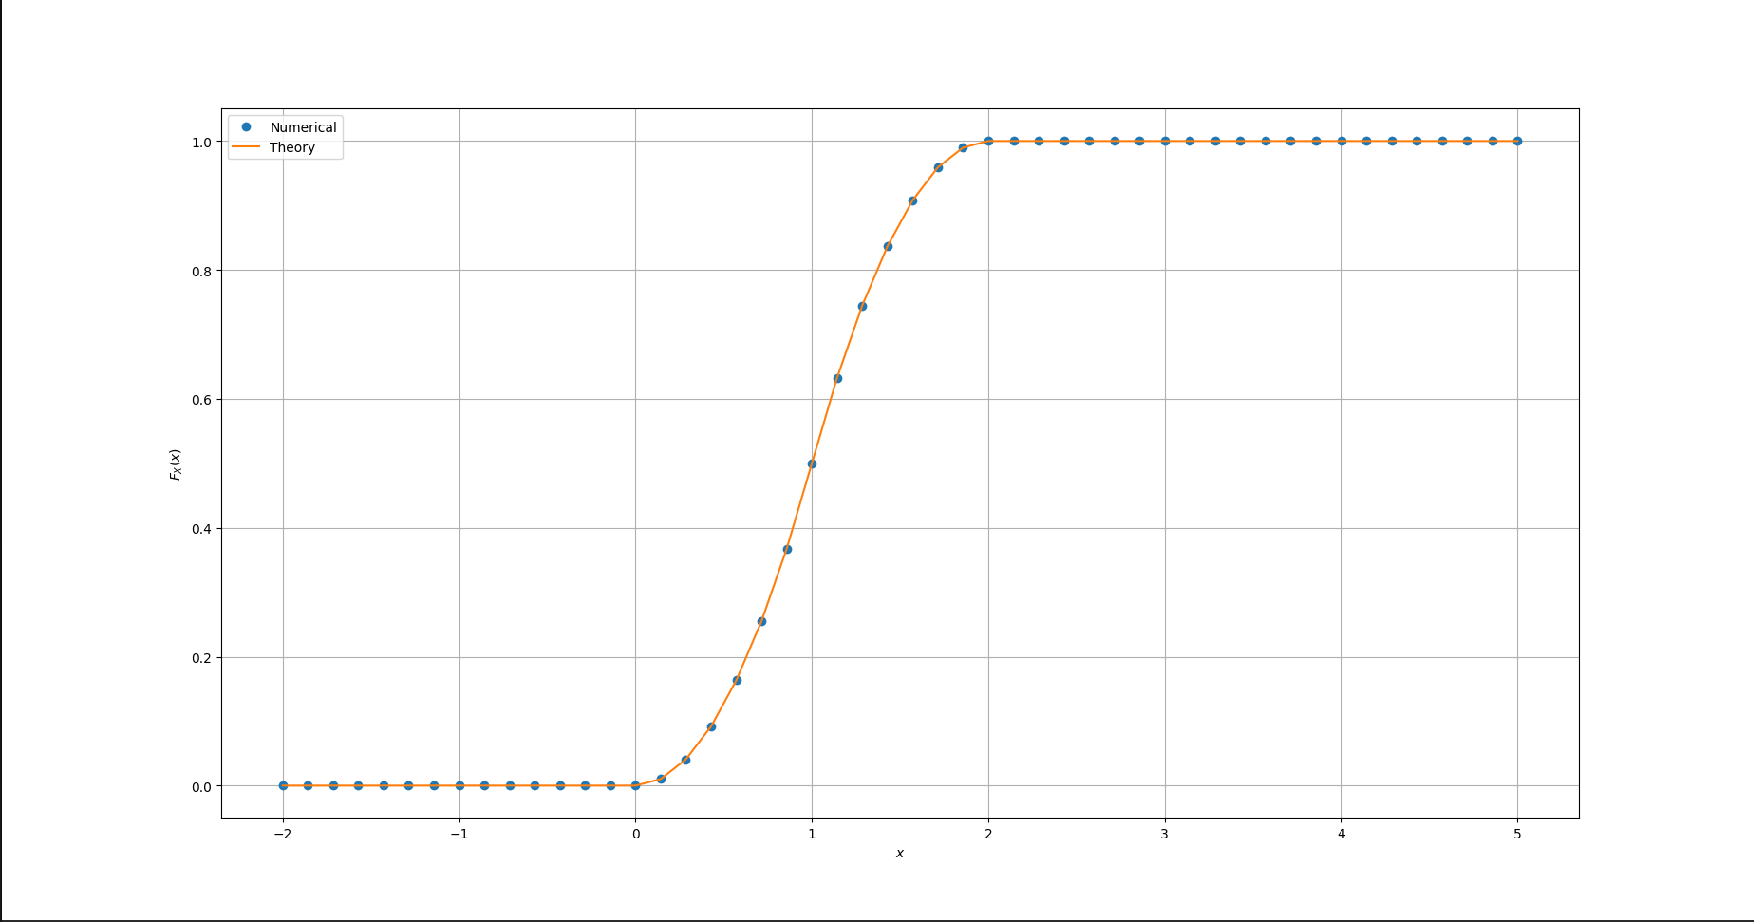
\includegraphics[width=0.5\textwidth]{T_cdf}
\caption{CDF for (4)}
\label{fig:T_CDF}
\end{figure}
Run the below code to get the cdf
\begin{lstlisting}
https://github.com/Ritvik-Sai-C/Random_numbers/blob/main/4.5/T_cdf.py
\end{lstlisting}
Use the following command in the terminal to run the code
\begin{lstlisting}
python3 T_cdf.py
\end{lstlisting}
\begin{figure}[h]
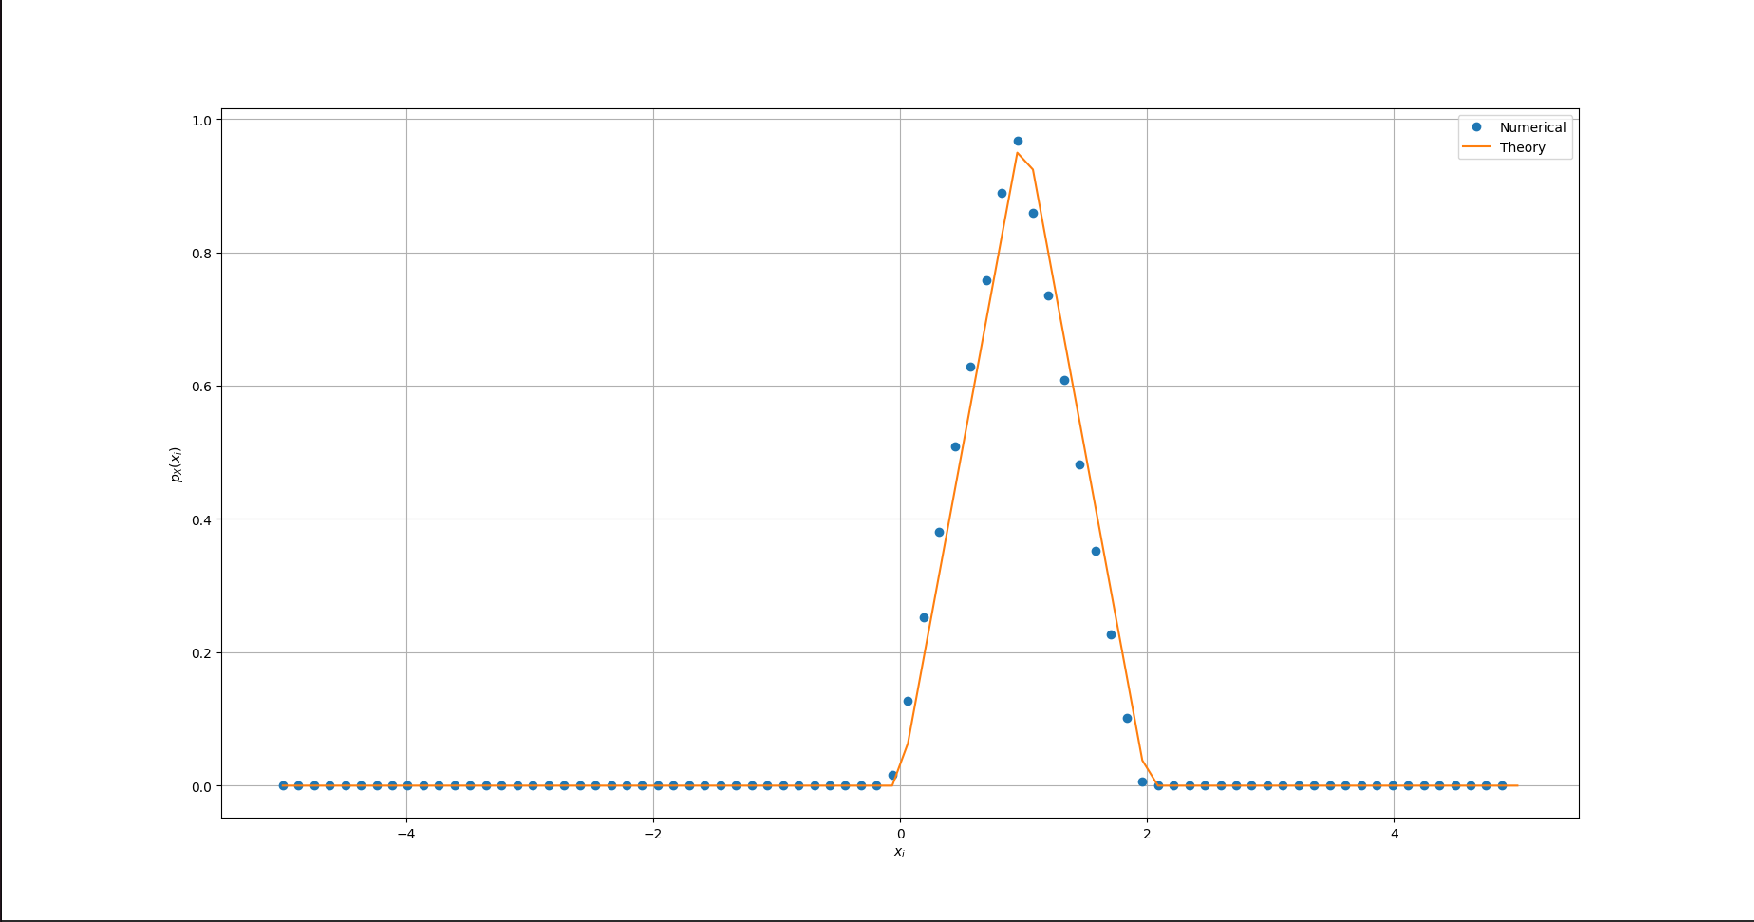
\includegraphics[width=0.5\textwidth]{T_pdf}
\caption{PDF for (4)}
\label{fig:T_PDF}
\end{figure}
Run the below code to get the pdf
\begin{lstlisting}
https://github.com/Ritvik-Sai-C/Random_numbers/blob/main/4.5/T_cdf.py
\end{lstlisting}
Use the following command in the terminal to run the code
\begin{lstlisting}
python3 T_pdf.py
\end{lstlisting}
\end{enumerate}
\section{Maximul Likelihood}
\begin{enumerate}[label=\thesection.\arabic*
,ref=\thesection.\theenumi]
\item Generate equiprobable $X \in \cbrak{1,-1}$.\\
\solution
Run the below code,
\begin{lstlisting}
https://github.com/Ritvik-Sai-C/Random_numbers/blob/main/5.1/bernoulli.c
\end{lstlisting}
Use the below command in the terminal to run the code
\begin{lstlisting}
gcc bernoulli.c -lm
./a.out
\end{lstlisting}
\item Generate 
\begin{equation}
Y = AX+N,
\end{equation}
		where $A = 5$ dB,  and $N \sim \gauss{0}{1}$.\\
\solution
Run the below code for generating samples of Y,
\begin{lstlisting}
https://github.com/Ritvik-Sai-C/Random_numbers/blob/main/5.2/Ygen.c
\end{lstlisting}
Use the below command in the terminal to run the code
\begin{lstlisting}
gcc Ygen.c -lm
./a.out
\end{lstlisting}
\item Plot $Y$ using a scatter plot.\\
	\solution
	\begin{figure}[h]
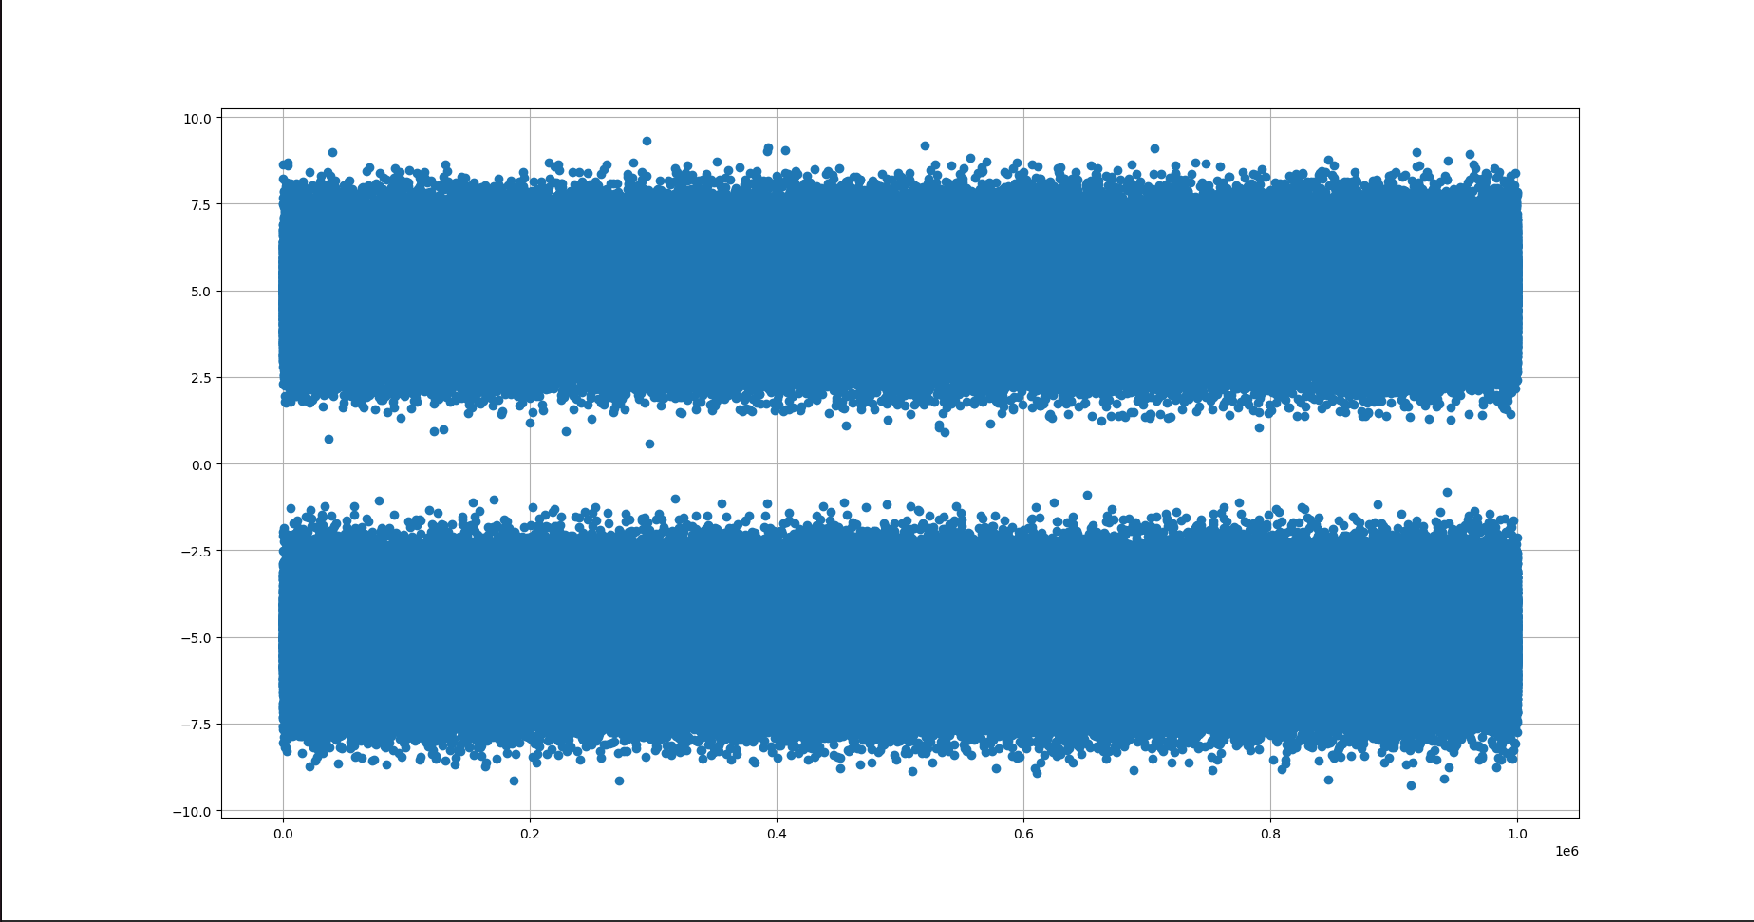
\includegraphics[width=0.5\textwidth]{Yplot}
\caption{plot for (5.3)}
\label{fig:Y_Plot}
\end{figure}
\\
	Run the following code to generate the scatter plot
	\begin{lstlisting}
https://github.com/Ritvik-Sai-C/Random_numbers/blob/main/5.3/Yplot.py
	\end{lstlisting}
	Use the below command to run the code,
	\begin{lstlisting}
     python3 Yplot.py 
	\end{lstlisting}
\item Guess how to estimate $X$ from $Y$.\\
	\solution
	if the received signal is greater than 0, then the receiver assumes $s_1$ was transmitted.\\
if the received signal is less than or equal to 0, then the receiver assumes $s_0$ was transmitted, where $s_0$ and $s_1$ are cases of $X=1$and $X=-1$ respectively where threshold 0 is taken to be the decision boundary.
\begin{align}
y>0 \implies s_1\\
y\leq 0 \implies s_0
\end{align}
\item
\label{ml-ch4_sim}
Find 
\begin{equation}
	P_{e|0} = \pr{\hat{X} = -1|X=1}
\end{equation}
and 
\begin{equation}
	P_{e|1} = \pr{\hat{X} = 1|X=-1}
\end{equation}
\solution 
Here $s_1$ and $s_2$ are equally probable ie, $p(s_1)=p(s_0)=\frac{1}{2}$ \\
\begin{align}
&Q(x)=\frac{1}{\sqrt{2\pi}} \int_{x}^{\infty} e^{\frac{-x^{2}}{2} } dx\\
&p(e|s_1)=\frac{1}{\sqrt{2 \pi}} \int_{-\infty}^{0} e^{-\frac{(y-A)^2}{2}} dy
\nonumber \\
&=Q(A)\\
&p(e|s_0)=\frac{1}{\sqrt{2 \pi}} \int_{0}^{\infty} e^{-\frac{(y+A)^{2}}{2}} dy
\nonumber \\
&=Q(A)
\end{align}
%
\item Find $P_e$ assuming that $X$ has equiprobable symbols.\\
\solution
Total probability of bit error:
\begin{align}
&P_{e}=p(s_1)p(e|s_1)+p(s_0)p(e|s_0)\\
&=\frac{1}{2}[Q(A)+Q(A)]\\
&\because p(s_1)=p(s_0)=\frac{1}{2},\text{X has equiprobable symbols}\\
\nonumber
&=Q(A)
&=Q(5) \because A=5
\end{align}
%
\item
Verify by plotting  the theoretical $P_e$ with respect to $A$ from 0 to 10 dB. \\
\solution
\begin{figure}[!ht]
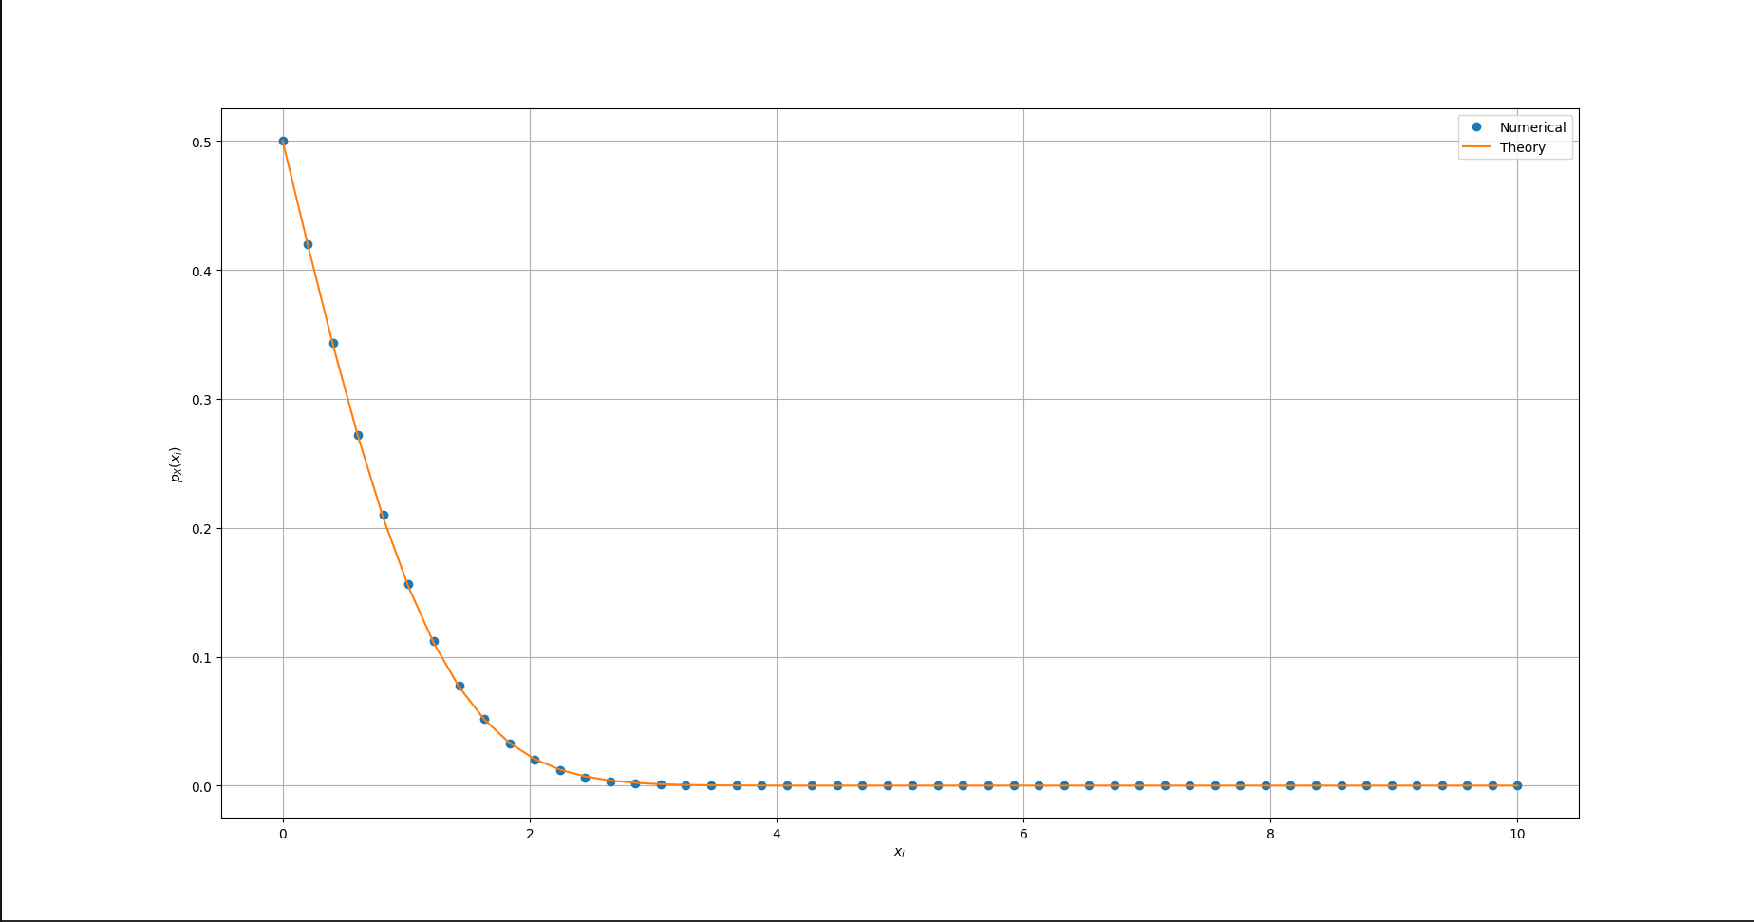
\includegraphics[width=0.3\textwidth]{Pplot}
\caption{plot for (5.7)}
\label{fig:Plt}
\end{figure}
	\begin{lstlisting}
https://github.com/Ritvik-Sai-C/Random_numbers/blob/main/5.7/Pplot.py
	\end{lstlisting}
	Use the below command to run the code,
	\begin{lstlisting}
     python3 Pplot.py 
	\end{lstlisting}
\item Now, consider a threshold $\delta$  while estimating $X$ from $Y$. Find the value of $\delta$ that minimizes the theoretical $P_e$.\\
\solution
Threshold=$\delta$, \\
\begin{align}
 &y>\delta \implies s_1\\
 &y \leq \delta \implies s_0\\
 &p(e|s_1)=\frac{1}{\sqrt{2 \pi}} \int_{-\infty}^{\delta} e^{-\frac{(y-A)^{2}}{2}} dy\\
 \nonumber
 &p(e|s_0)=\frac{1}{\sqrt{2 \pi}} \int_{\delta}^{\infty} e^{-\frac{(y+A)^{2}}{2}} dy\\
\nonumber
&P_e=\frac{1}{2\sqrt{2 \pi}}{( \int_{-\infty}^{\delta} e^{-\frac{(y-A)^{2}}{2}}dy+ \int_{\delta}^{\infty} e^{-\frac{(y+A)^{2}}{2}} dy)}\\
&P_e=\frac{Q(\delta+A)+Q(A-\delta)}{2}\\
&P_e=f(\delta)\\
&\text{to minimize} P_e, \frac{d(f(\delta))}{d\delta}=0 ~\text{and} f"(\delta)>0\\
&e^{\frac{-(A-\delta)^{2}}{2}}-e^{\frac{-(A+\delta)^{2}}{2}}=0\\
&\therefore A-\delta=A+\delta, \implies \delta=0\\
&f"(\delta)=k((A-\delta)e^{\frac{-(A-\delta)^{2}}{2}}+(A+\delta)e^{\frac{-(A+\delta)^{2}}{2}})>0
\end{align}
\item Repeat the above exercise when 
	\begin{align}
		p_{X}(0) = p
	\end{align}
\solution
 $p_{X}(0)=p$ \\
 $\implies p_{X}(1)=1-p$
 \begin{align}
 P_{e}=p P(e|s_0)+(1-p)P(e|s_1)\\
 =p Q(A+\delta)+(1-p)Q(A-\delta)\\
 \frac{d(P_{e})}{d(\delta)}=0\\
 \implies e^\frac{(A+\delta)^{2}-(A-\delta)^{2}}{2}=\frac{p}{1-p}\\
 \therefore \delta=\frac{1}{2A}log(\frac{p}{1-p})\\
  \frac{d(P_{e})}{d(\delta)}\quad at \quad \delta+\epsilon>0 \\
  \nonumber
   \frac{d(P_{e})}{d(\delta)} \quad at\quad \delta-\epsilon<0 \\
   \nonumber
   \therefore \delta=\frac{1}{2A}log\left(\frac{p}{1-p}\right)\longrightarrow   minima\\
   A=5 \implies \delta=\frac{1}{10}log\left(\frac{p}{1-p}\right)
 \end{align}
 \\
\item Repeat the above exercise using the MAP criterion. \\
\solution
\begin{align}
&P_{X|Y}\brak{x|y} \big|_{X=1}= \frac{P(Y=y|X=1)P(X=1)}{P(Y=y)}\\
\begin{split}P(Y=y)=P(Y=y|X=1)P(X=1)\\+P(Y=y|X=-1)P(X=-1)\end{split}\\
&P(Y=y|X=1)P(X=1)=p P(Y=A+N)\\
&=p\brak{\frac{1}{\sqrt{2 \pi}} e^{\frac{-(y-A)^2}{2}}}\\
&\therefore P_{X|Y}(x|y) \big|_{X=1}=\frac{p\brak{\frac{1}{\sqrt{2 \pi}} e^{\frac{-(y-A)^2}{2}}}}{P(Y=y)}\\
&P_{X|Y}(x|y) \big|_{X=-1}= \frac{P(Y=y|X=-1)P(X=-1)}{P(Y=y)}\\
&P(Y=y|X=-1)P(X=-1)=(1-p) P(Y=-A+N)\nonumber\\
&=(1-p)\brak{\frac{1}{\sqrt{2 \pi}} e^{\frac{-(y+A)^2}{2}}}\\
&\therefore P_{X|Y}(x|y) \big|_{X=-1}=\frac{(1-p)\brak{\frac{1}{\sqrt{2\pi}} e^{\frac{-(y+A)^2}{2}}}}{P(Y=y)}
\end{align}
Now comparing $a=P_{X|Y}(x|y) \big|_{X=-1}$ and $b=P_{X|Y}(x|y) \big|_{X=1}$, if $a>b, X=-1$ is more likely ,$a<b, X=1$ is more likely.\\
$p e^{\frac{-(y-A)^2}{2}}\gtrless(1-p)e^{\frac{-(y+A)^2}{2}}$\\
$\implies e^{2Ay}\gtrless\frac{1-p}{p}$\\
$\implies y\gtrless\frac{1}{2A}log\brak{\frac{1-p}{p}}$\\
$\delta=\frac{1}{2A}log\brak{\frac{1-p}{p}}$\\
$y>\delta \implies$ X=1 is more likely\\
$y<\delta \implies$ X=-1 is more likely
		\end{enumerate}
		\end{document}